\documentclass{article}
\usepackage{amsmath}
\usepackage{amssymb}
\usepackage{graphicx}
\usepackage{hyperref}
\usepackage[version=4]{mhchem}

\title{Problem 21}
\date{}

\begin{document}
\maketitle

\section*{Problem}
In parallelogram \(A B C D\), point \(M\) is on \(A B\) so that \(\frac{A M}{M B}=\frac{17}{1000}\), and point \(N\) is on \(A D\) so that \(\frac{A N}{N D}=\frac{17}{2009}\). Let \(P\) be the point of intersection of \(A C\) and \(M N\). Find \(\frac{P C}{P A}\).\\
\centering
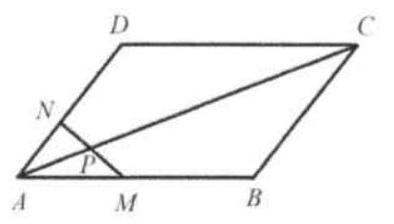
\includegraphics[width=\textwidth]{images/130(1).jpg}

\section*{Solution}
178.\\
Extend \(N M\) through \(M\) to \(E\) and to meet the extension of \(C B\) at \(E\). We label the line segments as shown in the figures.\\
We know that \(A D / / C E\). So \(\triangle A M N \sim \triangle B M E\) (Figure 1). \(\frac{A N}{B E}=\frac{A M}{M B} \quad \Rightarrow\)

\[
\frac{17 y}{B E}=\frac{17 x}{1000 x} \Rightarrow \quad B E=1000 y .
\]

We know that \(A N / / C E\). So \(\triangle A P N \sim \triangle C P E\) (Figure 2).\\
\centering
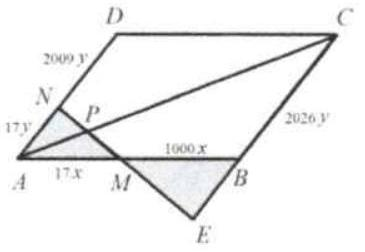
\includegraphics[width=\textwidth]{images/142(3).jpg}

Figure 1\\
\centering
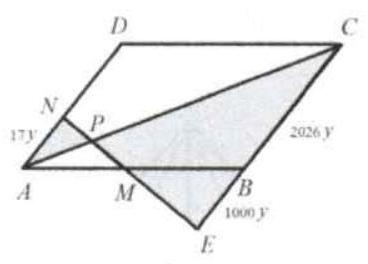
\includegraphics[width=\textwidth]{images/142.jpg}

Figure 2\\
\(\frac{P C}{P A}=\frac{C E}{A N}=\frac{2026 y+1000 y}{17 y}=178\).

\end{document}
